\documentclass[dvipsnames]{ctexbeamer}

\usepackage{bm}
\usepackage{mathtools}
\usepackage{stmaryrd}
\usepackage{color, xcolor}
\usepackage{tikz}
\usepackage{soul}
\usepackage{cancel}

\usetikzlibrary{arrows, positioning}

\usepackage{fourier}
\usepackage{nicefrac}
\usepackage{ulem}

\usepackage[
    type={CC},
    modifier={by},
    version={4.0},
    % imagemodifier={-80x15},
    lang={chinese-utf8},
]{doclicense}

% \usepackage[orientation=landscape,size=custom,width=16,height=9,scale=0.5,debug]{beamerposter}

\newtheorem{remark}[theorem]{注记}

\DeclareMathOperator{\mex}{mex}
\newcommand{\me}{\mathrm{e}}

\newcommand{\Gname}{三染色}
\newcommand{\sfT}{\mathsf T}

% \usetheme{Berkeley}
\usetheme{metropolis}
% \usecolortheme{spruce}
\usefonttheme{professionalfonts,structurebold}

\title{THUPC2024 初赛}
% \subtitle{Selected Topics in Graph Enumeration {\color{red} (draft)}}
\author{\textsc{Elegia}, \textsc{E\textperiodcentered Space}, \textsc{fzw}, \textsc{Itst}, \textsc{liuzhangfeiabc}, \textsc{SpiritualKhorosho}\textsuperscript{\textdagger}}
\institute{清华大学算法协会}
\date{2023 年 12 月 17 日}

\begin{document}

\frame{\titlepage}

\frame{
    除命题人外, 感谢~ \textsc{He-Ren}, \textsc{Mys.C.K.},\textsc{PinkRabbait} ~等人参与题目准备工作.

    \textsuperscript{\textdagger} 按照字典顺序排列.
}

% \section[Outline]{}
\frame[allowframebreaks]{
    \tableofcontents[sections={1-3}]
    \framebreak
    \tableofcontents[sections={4-6}]
}

\section{Part 0 (出题人 {\itshape liuzhangfeiabc})}

\subsection{M 你说得对,但是 AIGC}
\frame
{
  \frametitle{M 你说得对,但是 AIGC {by \itshape liuzhangfeiabc}}

	判断输入串的前 \texttt{19} 个字符是不是 `You are right, but `,是则输出 `AI`,否则输出 `Human`

}

\frame
{
	\frametitle{花絮}

	中文2字英文7字的游戏除了扫雷 Winmine,还有蔚蓝 Celeste,\sout{东方 Project}.

	第3个样例是应验题人的要求加上去的. \sout{出题人表示不知道“G****** I*****”是什么东西\tiny{(投降喵)}}

}


\section{Part I (出题人 {\itshape Elegia})}

\subsection{C 前缀和}
\frame
{
  \frametitle{C 前缀和 {by \itshape Elegia}}

  有一个 \texttt{0} 到 \texttt{1} 之间的实数 $p$,接下来生成 $n$ 个随机数,随机方式如下:\\
  每个 $x_i$ 独立生成,有 $p$ 的概率是 \texttt{1},$(1-p)p$ 的概率是 \texttt{2},以此类推.\\
  给定 $1\le l\le r\le n$,问序列 $\{x_i\}$ 的前缀和序列 $\{y_i\}$ 中,期望有多少个数落在 $[l, r]$ 之间?

}


\frame
{
    \frametitle{问题转化}

	考虑有无穷多个灯,编号从 \texttt{1} 开始一字排开,每个灯独立有 $p$ 的概率亮起,$1-p$ 的概率是灭的. \pause

	我们从左往右数,第一次找到一个灯的编号,这就是 $x_i$ 的分布,所以序列 $\{y_i\}$ 就是第 $i$ 个亮起的灯的位置. \pause

	所以问题就是在问:$[l, r]$ 之间,期望有多少亮起的灯?\pause

   	答案就是 $(r-l+1)p$.
}


\subsection{I 分治乘法}
\frame
{
    \frametitle{I 分治乘法 {by \itshape Elegia}}



    有三种构造集合的方式:

  \begin{itemize}
  \item 创建一个集合 $\{x\}$
  \item 将两个不交集合 X, Y 合并
  \item 将集合平移 X + y
  \end{itemize}

  之前构造的集合可以重复使用.

  构造的总代价是构造出的所有集合大小之和.

  一个数均不超过 $5 \times 10^5$ 的集合,用不超过 $5 t\times 10^6$ 的代价构造出它.

}

\frame
{
    \frametitle{两个初步的思路}

    不能直接按照标题分治吗? \pause
    \begin{itemize}
    \item 按照题目的要求计算,分治的代价大概是 $N \lg N$,要比题目限制多出一倍. \pause
    \end{itemize}
    什么样的集合能借助平移操作显著快速地构造? \pause

    \begin{itemize}
    \item 考虑 $[1, n]$,可以先构造出 $\left[1, \frac{n}{2}\right]$,再平移,如果需要的话再补上最后一个元素.
    \item $T(N) = T\left(\frac{N}{2}\right) + O(N)$ 最后总代价还是 $O(N)$. \pause
    \end{itemize}
    如何将二者有效地结合?

}

\frame
{
    \frametitle{四毛子}

    考虑设置一个块大小 $L$,将集合剖成 $\frac{N}{L}$ 个大小为 $L$ 的块.

    一个块有 $2^L$ 种可能性,我们记每种可能性的块构成的集合为 $S_i$. \pause

    所有 $S_i$ 的大小总和是 $\frac{N}{L}$,我们先构造出每个 $S_i$,然后平移出它在原序列中的 $S_i+x$,这一步的总代价是 $\frac{N}{L}\log_2 N + N$. \pause

    现在我们要合并 $L2^L$ 个集合,把它们用 Huffman 树合并,代价是 $N \log_2 (L2^L) \sim NL$. \pause

    取 $L=\sqrt{\log_2 N}$,总代价是 $O(N\sqrt{\log_2 n})$.
}

\frame
{
	\frametitle{常数}

	上面这个做法取 $L=5$,挂在 Huffman 树上跑,我能构造出来的数据基本上代价最多也就是 $3.8 \times 10^6$ 的代价.

	我用了一些手段严格证明了这个做法在数据范围内是严格正确的(代价不超过 $4.9 \times 10^6$),所以开了这个数据范围,具体的不等式放缩赛后公开, \sout{跑了一个 L 个变量的凸优化}. \pause

	似乎这个问题还有很多其他奇怪的做法也很有希望卡到数据范围之内(而且这个数据范围看起来很像卡常),所以实际上可能八仙过海了.

	欢迎交流可以证明更低的代价复杂度的做法!


}

\subsection{J 套娃}
\begin{frame}{J 套娃 {by \itshape Elegia}}
	给一个序列 $a$,对每个 $k$,询问
	\begin{itemize}
	\item 把所有长为 $k$ 的子区间求 mex,对得到的答案集合再取 mex
	\end{itemize}
	的结果.


\end{frame}

\begin{frame}{解法}
	首先考虑所有里层的 mex 的数会如何出现. \pause

	如果一段区间的 mex 值是 $v$,那么这个区间首先不存在一个值域为 $v$ 的数,然后 $0,...,v-1$ 这些数都出现过. \pause

	我们首先考虑数列中所有出现过的数字 $v$,它们出现过的位置将这个序列分割成 $c_v$ 段(我们有 $\sum c_v=O(n)$),mex 值是 $v$ 的段肯定只能是其中某一段的子区间. 而且如果某一段里存在的话,那么这一整段肯定存在,所以有一个长度区间 $[d, u]$,表示 $d,...,u$ 这些长度都有作为 $v$ 的 mex 存在过.

\end{frame}


\begin{frame}{解法}
	如果处理出了这些 $[d, u]$,我们只需要扫描线一下就就可以求出要输出的所有答案了,复杂度 $O(n \log n)$. \pause

	接下来考虑如何确定这些 $[d, u]$。从小到大考虑 $v$,对于每个 $i$ 我们维护一个最小的数 $p_i$ 表示 $[i, p_i]$ 里出现过所有 $0,...,v-1$ 的数, 那么 $p_i$ 这个阶梯型可以用线段树维护. \pause

	查询被 $v$ 分割出的一段 $[l, r]$ 里最小的区间时, 我们先想办法二分出最大的 $i$ 满足 $p_i < r$,然后用线段树顺带维护出 $p_i - i + 1$ 的最小值,对此区间查询. \pause

	复杂度 $O(n \log n)$.


\end{frame}


\section{Part II (出题人 {\itshape E.Space})}

\subsection{E 转化}
\frame
{
 	\frametitle{E 转化 {by \itshape E.Space}}

	本题改编自桌游 Gizmos 的部分玩法,定位简单题.

	有 $n$ 种球,第 $i$ 种有 $a_i$ 个.
	\begin{itemize}
	\item 可以把 $i$ 变成任意颜色不超过 $b_i$ 次.
	\item 可以把 $i$ 变成两个 $i$ 不超过 $c_i$ 次.
	\end{itemize}

	对每个 $i$ 分别求最多能有多少个 $i$,以及求最多能有多少个球.

}
\frame
{
	\frametitle{正解}

	首先对于同一种颜色,$x+1$ 个第一种工具和 $x$ 个第二种工具可以组合起来用,把一个 $i$ 变成 $x+1$ 个任意颜色. \pause

	对于存在这样的组合的颜色,如果 $a_i\neq 0$,那么可以用原来的球直接变出 $x+1$ 个任意颜色,否则如果有任意颜色的球,可以用一个任意颜色的球变出来. \pause

	如果组合后有剩下的第一种工具和对应颜色的球,那么就可以用这些再变几个任意颜色的球. \pause

	所以第一问答案就是这种颜色剩下的球的数量加上任意颜色球的数量加上剩下的第二种工具的数量,需特判前二者均为 \texttt{0} 的情况.
}

\frame
{
	\frametitle{正解}

	对于第二问,显然如果 $a_i\neq 0$ 或者用过第 $i$ 种颜色的组合,那么所有关于第 $i$ 种颜色的第二类工具都会用上. \pause

	此外,如果还有剩下的第一类工具($a_i=0$ 且 $b_i=1$ 的情况),且有任意颜色的球,那么可以免费利用第一类工具转化而用上所有的第二类工具. \pause

	剩下的情况($a_i=b_i=0$)需要按照 $c_i$ 从大到小排序,每用一个颜色的工具就要消耗一个任意颜色的球.

}

\frame
{
	\frametitle{花絮}

	还是写题解的时候最清醒.

	我在写题解的时候发现了 std 的 bug 并加强了数据.

	还是验题人 Itst 比较厉害,一次就写对了.

}

\subsection{F 机器人}
\begin{frame}{F 机器人 {by \itshape E.Space}}

	一堆机器人.

	每个机器人有两只手和一些指令.

	求执行指令的过程与结果.

	题目定位是模拟题.

\end{frame}

\begin{frame}{正解}

	有几点需要注意. \pause

	指令不能直接深拷贝(可能很长),因此修改的时候不能直接在原来的指令上改(可能有别的指令包含这部分). \pause

	然后就没了. \pause

	指令可以用一个东西打包一下,验题人 zyb 用了下标指针+操作时判断类型,我写的是类继承+虚拟函数. \pause

	我的写法会更长一些,不过 VS Code 的根据声明自动生成定义还是好用的.

\end{frame}


\subsection{G 采矿}
\begin{frame}{G 采矿 {by \itshape E.Space}}

	一棵有根二叉树,初始有个机器人在 $s$.

	有 4 种指令:

    \begin{enumerate}
	\item 将机器人往祖先移至少一步
	\item 将机器人往子树里移至少一步
	\item 将一个人类加到根
	\item 将一个人类从根移走
	\end{enumerate}
	移动时只能点上站人且一个点只能包含不超过一个人.

	每个点有产出,根据上面的工人,在每个指令结算.

	指令之间人类可以任意移动,求最大总产出.


\end{frame}

\begin{frame}{正解}

	当前状态只和机器人位置、当前是哪个计划,以及被机器人分开的每个连通块里有几个人类有关. \pause

	全部记录到状态里暴力 DP. \pause

	注意每个时刻人类总数是已知的,所以只要记录两个子树里分别有多少人类. \pause

	状态总数为对每个点计算两个子树 size 的积加起来,是平方的. \pause

	前两种计划需要额外记录机器人是否移动过. \pause

	转移的时候需要枚举下一步往里走的那个子树里的人类怎么分配. \pause

	可以用前缀和优化做到 $O(1)$ 单次转移,总复杂度 $O(qn^2)$

\end{frame}

\begin{frame}{花絮}

	这题是我两年前看着堵死的停车位出的.

	改着改着就成这样了.

	虽然看着题目描述很像桌游说明书,但这题和桌游没有一点关系.

\end{frame}

\section{Part III (出题人 {\itshape fzw})}

\subsection{B 一棵树}
\frame
{
  \frametitle{B 一棵树 {by \itshape fzw}}

	树,选 $k$ 个点染黑,代价为边权求和,边权定义为两边子树黑色节点之差。
	
	$n,k\le 5\times 10^5$
}

\begin{frame}{正解}

	注意到当前询问形如权值为边权的权值求和,考虑树形 dp,直接的 dp 为 $f_{i,j}$ 表示 $i$ 子树内有 $j$ 个黑色节点的最小代价. \pause

	有转移是易于计算的,子树的合并是树形背包的合并 $f_{x,j+k}=\min(f_{x,j}+f_{to,k})$,考虑当前点 x 到父亲这条边的代价是多少. \pause

	注意到,形如如果当前子树有 $A$ 个黑点,子树外有 $k-A$ 个白点,代价为 $|2A-k|$.

\end{frame}

\begin{frame}{正解}

	观察函数的形式,你注意到如果将 $x$ 坐标作为黑点个数,$y$ 坐标作为代价,则每次代价增量为一个下凸函数,有树形背包合并不影响函数凸性. \pause

	注意到凸函数的维护可以尝试维护其差分数组,两个下凸函数做 $\min$ 卷积可以之际的视作差分数组的归并. \pause

	现在需要考虑的问题是往父亲方向的增量怎么处理.

\end{frame}

\begin{frame}{正解}

	考虑代价增量的差分,形如一段前缀差分为负数,一段后缀差分为正数,中间一个点根据 k 的奇偶性讨论是否存在差分 = 0. \pause

	有这一段前缀的长度总为定长度 $\lfloor \frac k 2 \rfloor$ 于是我们维护可并堆顶堆,使得左侧堆大小始终为前缀定长度,然后可以打加法标记实现. \pause

	总复杂度 $O(n\log n)$.

\end{frame}


\subsection{H 二进制}
\begin{frame}{H 二进制 {by \itshape fzw}}

	01串,顺序枚举数 i 然后作为二进制串,在原串中找到并删除,需要返回是否可行以及可行时出现次数。

	$n\le 10^6$

\end{frame}

\begin{frame}{正解}

	观察到当前过程形如你需要每次维护使得可以查找某些子串出现次数与位置,尝试观察询问,注意到查找子串的长度不会超过 $\log_2 (n)$. \pause

	我们对于每个二进制数都维护这个数在原串中的出现位置,注意到当前形如只需要检查原串的长度为 $\log_2(n)$ 的子串. \pause

	每次删除后我们需要重新检查删除这一段和前后 $\log_2(n)$ 个元素,每次检查加插入总复杂度为 $\log_2^3(n)$. \pause

	注意到,执行删除操作的次数不会超过 $\frac n{\log_2(n)}$ 有总复杂度在 $n\log_2^2(n)$ 级别. \pause

	由于常数极小,所以可以直接通过。

\end{frame}


\section{Part IV (出题人 {\itshape Itst})}

\subsection{A 排序大师}
\frame
{
  \frametitle{A 排序大师 {by \itshape Itst}}
	用最少的 "段交换" 操作将长度为 $n$ 的排列排序。
	
	"段交换" 操作为以下操作:将排列分成五段,其中第二段和第四段不能为空、其他段可以为空,交换第二段和第四段再拼回去。

	$n\le 2000$.
}

\begin{frame}{正解}

	需要最小化交换次数,意味着我们同时需要上界和下界的分析.

	下界分析的常用办法是图模型,最常见的是 $p_i\rightarrow i$ 的模型. 但对于这个操作来说它不适用,因为一次交换会导致图上很多的边产生改变. \pause

	这提示我们需要考虑这样的图模型:在这个模型下,一次段交换操作只会改变其中常数条边.

	再注意到,一次交换中形如 $p_i\rightarrow p_{i+1}$ 的边只会改变最多四条,符合我们的要求,但这个模型并不能直接用于下界分析,因为目标状态是一条特殊的链,不能用环数分析.

\end{frame}

\begin{frame}{正解}

	我们做一些简单的调整:在排列最前面加入一个 $0$、最后加入一个 $n+1$,然后加入 $p_i\rightarrow p_{i+1}$ 的边。此时终态是一个 ${n+1}$ 个自环构成的图,符合“单次操作改变边数少”,同时环数相关的下界分析可以利用了.

	此时我们来考虑一次操作究竟会干什么.

\end{frame}

\begin{frame}{正解}
	不妨假设第三段非空,此时交换前后的状况如下:

	\centering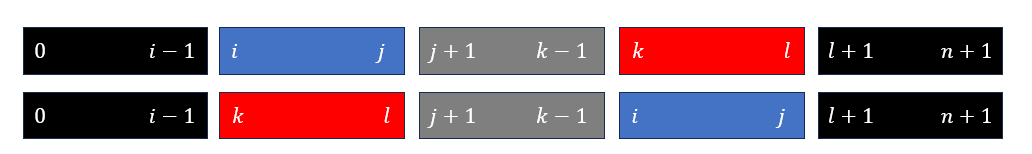
\includegraphics[width=\textwidth,keepaspectratio]{sources/A1.jpg}

	最初的四条边


$p_{i-1}+1\rightarrow p_i, p_j+1\rightarrow p_{j+1}, p_{k-1}+1\rightarrow p_k, p_l+1\rightarrow p_{l+1}$

 	被改为

$p_{i-1}+1\rightarrow p_k, p_l+1\rightarrow p_{j+1}, p_{k-1}+1\rightarrow p_i, p_j+1\rightarrow p_{l+1}$

	看起来还是画图比较直观(

\end{frame}


\begin{frame}{正解}

	\centering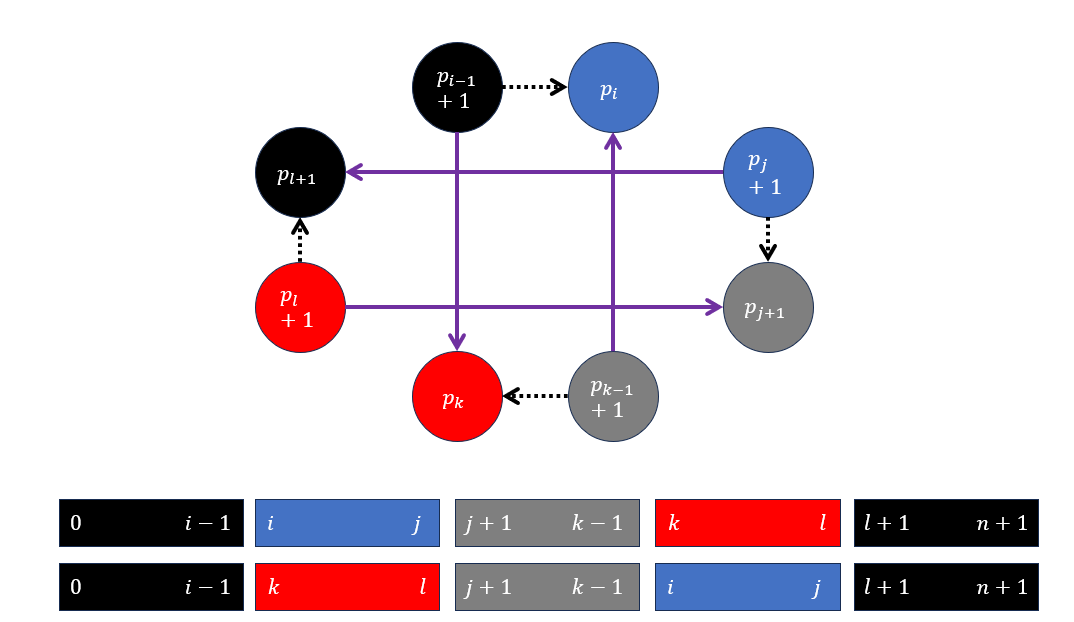
\includegraphics[width=\textwidth,keepaspectratio]{sources/A2.jpg}

\end{frame}

\begin{frame}{正解}

	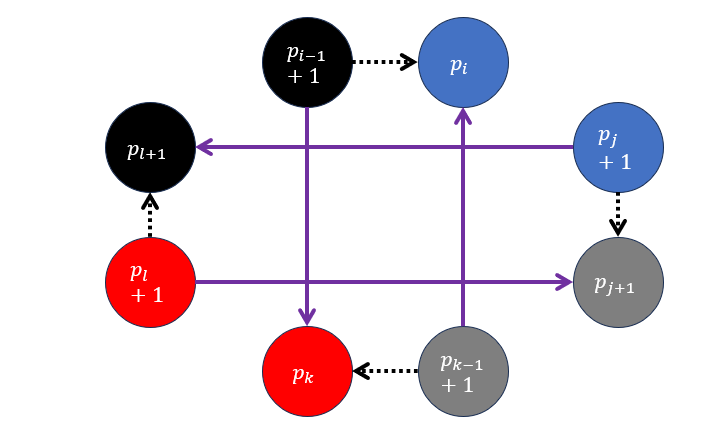
\includegraphics[width=0.8\textwidth,keepaspectratio]{sources/A3.jpg}

	这个修改操作相当于做以下操作两次:

	\begin{itemize}
	\item 选两条边交换它们的出点
	\end{itemize}

	这个操作会恰好将环数改变 \texttt{1}(读者自证不难),因此一次操作最多将环数减少 \texttt{2},且不会改变环数的奇偶性。

\end{frame}

\begin{frame}{正解}

	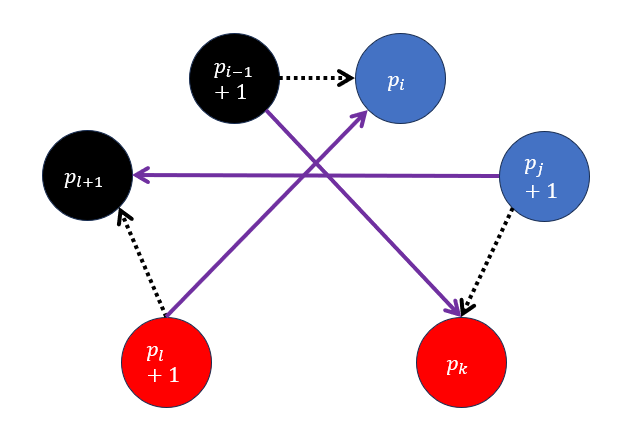
\includegraphics[width=0.8\textwidth,keepaspectratio]{sources/A4.jpg}

	对于第三段为空($j+1=k$)的情况,可以认为是先交换了 $p_{i-1}+1$ 和 $p_j+1$ 的出边,再交换 $p_j+1$ 和 $p_l+1$ 的出边,所以环数也最多改变不超过 \texttt{2},且不改变环数奇偶性。

\end{frame}

\begin{frame}{正解}

	因此我们只要能找到一种操作方案每次将环数增加 2 就行了。

	考虑如下构造:

	 \begin{enumerate}
	\item 选择一个最小的 $x$ 满足 $x$ 前面有比 $x$ 大的元素
	\item 再选择 $x$ 前面最大的元素 $y$
	\item 此时 $x-1$ 一定在 $y$ 前面(否则与 $x$ 的最小性矛盾),且 $y+1$ 一定在 $x$ 后面(否则与 $y$ 的最大性矛盾),因此用一次操作将 $x-1,\cdots, y, \cdots, x, \cdots, y+1$ 变为 $x-1, x, \cdots, y, y+1$
	\end{enumerate}

\end{frame}

\begin{frame}{正解}

	在  $x-1,\cdots, y, \cdots, x, \cdots, y+1$  中被修改的四(或三)条边为与 $x$ 相邻的两条边和与 $y+1$ 相邻的两条边,所以这四(或三)条边一定在一个或两个环里.

	而修改过后,出现了额外的两个自环($x-1, x$ 以及 $y, y+1$)。因为环数奇偶不会改变,因此环数一定加 \texttt{2}. \pause

	\sout{当然也有一些其他的构造可能满足以上条件.}\\ \sout{所以这题正确的做法是,猜一堆结论,写个 gen 拍一拍,拍过了就交.}


\end{frame}


\section{Part V (出题人 {\itshape SpiritualKhorosho})}

\subsection{D 多折较差验证}
\frame
{
  \frametitle{D 多折较差验证 {by \itshape SpiritualKhorosho}}

  	对于 $w=w_1 w_2 \cdots w_L \in \left\{\land, \lor\right\}^L (L\ge 0), \alpha \in \left\{\land, \lor\right\}$,称具有形式 $w + \alpha + \bar{w}$ 的折痕序列是可以沿着 $\alpha$ 恰好重合地折叠的,其中
	$\bar{w} = \bar{w}_L \bar{w}_{L-1} \cdots \bar{w}_1$,而对单个字符有 $\bar{\land} = \lor, \bar{\lor} = \land$。

	对于任意的折痕序列 $w = w_1 w_2 \cdots w_M$,称 $w$ 可以在 $w_k$ 处折叠,当且仅当:
	\begin{itemize}
		\item 若 $k\le (M+1)/2$,则 $w_1 \cdots w_{2k+1}$ 可以沿着 $w_k$ 恰好重合 地折叠;折叠后得到 $w_{k+1} \cdots w_L$,不对称程度 $L - 2k - 1$。
		\item 若 $k> (M+1)/2$,则 $w_{2k-L} \cdots w_L$ 可以沿着 $w_k$ 恰好重合地折叠;折叠后得到 $w_1 \cdots w_{k-1}$,不对称程度 $2k-L-1$。
	\end{itemize}

	给出折痕序列 $s_1 s_2 \cdots s_N \in \left\{\land, \lor\right\}$,求出将该序列折叠成空串的最小操作次数,并求出在此前提下最小的不对称程度之和。

	$1\le N\le 5000.$
}

\begin{frame}{分析}
	
	题目中描述的折叠过程具有最优子结构的性质,这启发我们使用区间 DP 进行求解.

	记 $Check(l, r, k) = 1$ 表示 $s_l \cdots s_r$ 可以在 $s_k$ 处折叠,$Check(l, r, k) = 0$ 表示不可以这样折叠;$f(l,r) =(x,y)$(此处有序数对根据字典序比较)表示对 $s_l, \cdots, s_r$ 进行折叠时,最小的折叠次数为 $x$,且此时最小的不对称程度为 $y$.

	对于每个 $f(l,r)$,直接枚举$k$ 并判断是否 $Check(l,r,k)=1$ 再进行转移是 $O\left(N^3\right)$ 的,显然不能通过本题.

\end{frame}

\begin{frame}{优化转移}
	
	为此,考虑优化枚举 $k$ 的过程:从枚举所有 $k$ 改为只枚举满足重合要求的 $k$。

	为了实现这个优化,需要分别对每个 $i$ 做左端点或右端点的情况,求出有哪些 $k$ 恰好可以覆盖到端点 $i$。计算 $f(l,r)$ 时,对区间左侧枚举可以覆盖到 $l$ 的折痕 $k$,使用 $f(k+1,r)$ 进行转移;对区间右侧枚举可以覆盖到 $r$ 的折痕 $k$,使用 $f(l,k-1)$ 进行转移。\pause

	然后你会发现,你可以通过本题。

\end{frame}


\begin{frame}{复杂度?}
	
	优化后的做法的复杂度分析比较复杂\sout{,反正出题验题人都不会}。与回文串及回文半径不同的是,这里取反后对称的规定使得有效的转移次数不会很多。例如,如果在一棵完全二叉树中任意结点的左右子树都是反对称的,那它的中序遍历可以将转移次数卡到 $O\left(N^2 log N\right)$。部分测试数据是根据这个思路生成的,但出题人及验题人不确定是否有更强且规则较为简单的数据形态.

	如果有选手可以证明本题的转移次数是 $O(N^2 \log N)$ 的,或者举出不满足这一复杂度的数据构造方式,都欢迎提出.

\end{frame}

\subsection{K 三步棋}
\frame
{
  \frametitle{K 三步棋 {by \itshape SpiritualKhorosho}}

  	给定一个在 $5\times 5$ 的棋盘上进行的简单双人零和完全信息有限博弈.

	初始状态是否为先手必胜取决于给出的 "由不超过 $4$ 枚棋子组成的四连通图案".

	$T$ 组数据,每次给出一个图案,询问是否为先手必胜.
}

\begin{frame}{分析}

	棋盘只有 $5\times 5$,可以考虑记忆化搜索。对任意给定局面,枚举当前操作的玩家将棋子摆在哪个位置,递归求解.

	然而直接记忆化搜索,计算量大概是 $2^{5^2}\times 5^2$ 级别的,再加上多组数据显然无法直接通过.

\end{frame}

\begin{frame}{我会打表!}

	注意到本题保证图案最多包含 $4$ 枚棋子,且本题的规则具有很强的对称性,本质不同的输入只有如下几种:

	\begin{itemize}
	\item 恰有 $1$ 枚棋子,仅 $1$ 种可能性;
	\item 恰有 $2$ 枚棋子,同样只有 $1\times 2$ 这 $1$ 种可能性;
	\item 恰有 $3$ 枚棋子,分为 $1\times 3$ 和 L 形两种;
	\item 恰有 $4$ 枚棋子,可以参考俄罗斯方块,合并旋转对称的 $2$ 对后只有 $5$ 种.
	\end{itemize}

	恰有 $1$ 枚棋子的情况显然;样例中给出了 $1\times 2$ 和 $1\times 3$ 的两种情况的答案,故只需要再打表剩余的 $6$ 种即可.\pause

	精心挑选了一种不能直接根据棋子数量输出答案,但又不会太复杂的规则,希望大家能喜欢.

\end{frame}

\subsection{L 勇闯末日塔}
\frame
{
  \frametitle{L 勇闯末日塔 {by \itshape SpiritualKhorosho}}
	在一个球面上有 $N$ 个点 $M$ 条弧,保证弧无重边自环,所有弧构成连通无向图,且弧各不相交. 每条弧对应容量 $w_i$(需要根据弧长计算).

	给出源 $s$ 和汇 $t$,求删去恰好 $L$ 个点后从 $s$ 到 $t$ 最大流的最小值.

	$3\le N \le 1000, 1\le L \le \min\{8, N-2\}$

}

\begin{frame}{M 的范围}
	虽然原题中数据范围给的是 $2\le M\le \frac{N(N-1)}{2}$,但显然数据中的 $M$ 不会很大. \pause

	注意到弧在球面上互不相交这一强保证,输入的图其实是一张平面图。根据平面图的知识可知,$M\le 3N-6$. \pause

	当 $N$ 个点的位置给定时,实际的最大边数可能受球面上的弧互不相交的影响,达不到 $(3N-6)$ 的上界. 但无论如何,$M\le 3N-6$.
\end{frame}


\begin{frame}{如何求平面图的最大流?}

	众所周知,最大流等价于最小割.

	对于平面图而言,最小割相当于一条在对偶图上横穿原图中的边的最短路\sout{(你可能想找:狼抓兔子)}.

	在球面上的情况也是类似的,只是此时应求一条将 $s$ 和 $t$ 所在球面分开的最短环.

\end{frame}

\begin{frame}{如何删点}

	原来投这个题的时候 $L=1$,可以枚举要删哪个点,然后从这个点出发,走向相邻的面(对偶图的点),再走对偶图最短路回到这个点。所有 $(N-2)$ 条对偶图最短路的最小值即为答案.

	注意这里最短路要考虑是否能把 $s$ 和 $t$ 分割开。在平面上的类似问题的常见解决办法是,挑选一条射线,并要求路径穿过射线奇数次。在本题中,比较难画出球面上的一条线并进行判断;一种可行的处理办法是,通过 BFS 任取一条从 $s$ 到 $t$ 的原图中的路径,并要求求出的环需要恰好经过这条路径奇数次.

	为什么不出 $L=1$?因为 $L=1$ 的时候删点跑最大流可以过.

\end{frame}


\begin{frame}{如何删点}

	对于 $L$ 更大的情况,可以把已确定删掉的点的数量记在状态里面。如果有一个原图中的点 $v$ 要删掉,相当于可以不使用对偶图中的边权,从原图中与 $v$ 相邻的面走到 $v$,再走到与 $v$ 相邻的另一个面。(注意删除的点数归在其中一种转移进行计算)

	此时仍需要枚举一个初始点跑广义最短路(或者说 DP)。注意到从面到面走对偶图中的边、从面到点或者从点到面走辅助的 $0$ 权边的转移次数都是与 $M$ 相关的(对于枚举的每个初始点,转移次数是 $O(ML)$ 的),总复杂度为 $O\left(N^2 \log N\right)$ 。

\end{frame}

\begin{frame}{剪枝}

	前述朴素实现即可通过本题,但我们还可以再优化,因为显然需要经过一个与通过 BFS 预先确定的折线相邻的边.

	经测试,加了剪枝的 SPFA 只跑了 0.2s,所以时限还是相当宽松的.

\end{frame}

\begin{frame}{致谢}

	感谢小 E 提供加强后的做法.

	感谢家里的冰箱为这道题保鲜.

\end{frame}



\begin{frame}{}
    \begin{center}
        \Large 感谢倾听!
    \end{center}
\end{frame}

\end{document}
